% background and related work 
% material science 
% our work 

%The creation of large collaborative projects such as the Materials Genome Initiative~\cite{material_genome_initiative}, contributed to accelerate the change, however the amount of structured data represent a negligible part of the potentially available information.

%At the moment, the only available database for superconducting material discovery is Supercon, which is old, small (only 30000 entries) and outdated. There is needs of modernising or rebuilding the current manual process, which cannot keep-up with the current publication rate. 
% We are currently working on a collaborative project to implement a system for mining information from superconductors-related literature using different approaches of machine learning and rule-based. 

% We annotated entities such as materials, classes, measurement methods, and properties such as superconducting critical temperature values and expressions, and critical pressure. We linked materials with critical temperature, pressures, and measurement methods. 

%to accelerate toward breakthrough by exploiting the vast knowledge hidden in scientific literature. 

% The National Institute for Materials Science (NIMS) has been investing in establishing TDM processes to support material discovery. 
% manually constructing several databases to support materials research, and SuperCon\footnote{\url{http://supercon.nims.go.jp}} was a hopeful data source for superconductor domain. 


%For example, to help researchers retrieving information based on very granular search queries, to extract structured datasets automatically, or to aggregate information by semantic similarity. suitable to be the input data of deep analysis processes   or properties prediction (curie temperature, magnetocaloric temperature, etc...).

% [END]
% -- 

% [OLD] Data-driven science has become as the fourth dimension in scientific exploration, after experimentation, theory and simulation~\cite{doi:10.1063/1.4944682}.


% [OLD] The emergence of Machine Learning (ML), a sub-field of Artificial Intelligence (AI), followed by a growing infrastructure of tools for generating, testing, and refining scientific models give us some hope. Such approach allow to address complex problems which conventional techniques cannot solve efficiently. 

% Introduce the importance of high-quality training data 
% [OLD] On the other hand the development of statistical models require a solid base where to build more complex systems. Low quality or incorrect data, will propagate and exponentially impact on the out result. One of the dogma of text processing is "Garbage in, Garbage out", therefore is foremost important to reduce at minimum the "Garbage in" by having high quality data. 


% to be rephrased
%Contrary to what might seem like the conventional machine learning mantra, throwing more data at the problem is not always the solution. Instead, the quality and domain-specificity of the corpus determine its effectiveness for domain-specific tasks.

% In the field of superconductors materials, the manual data collection used to populate SuperCon\footnote{\url{http://supercon.nims.go.jp}} cannot cope with the massive fresh information from the increasing number of articles published every year. In addition, the current process cannot easily scale infinitely, for physical and economical constraints. 
%- 

%-

% A project is currently ongoing, and aims to develop a system for automatic superconductors database creation. From large quantities of superconductors{-}related articles, it aims to extract, automatically, superconductors material and their relative properties~\footcite{foppiano2019proposal}. 

% The dataset provides scientific text annotated with entities and relationship information (links). The entities are identified among 6 classes (or labels) as summarised in Figure~\ref{fig:classes_frequency} and linked using relationships \texttt{material-tc} and \texttt{tc-pressure} (Table~~\ref{tbl:summary-links}). 

% This corpus is designed for training sequence labelling statistical models and can be utilised for developing domain-specific systems for entity extraction, entity-relationship and clustering. 

%Recently, however, thanks to large collaborative projects such as the Material Genome Initiative~\cite{material_genome_initiative}, the data-driven approach gained popularity. 
%The term Materials Informatic (MI) is used for defining the sub-domain dedicated to computational discovery. 
%Unfortunately, the number of structured material data still represents a negligible part of the available knowledge. 
%Most of them, such as AFlow~\cite{CURTAROLO2012218}, Polynfo~\cite{polynfo}, the Pauling File~\cite{Blokhin2018ThePF_paulingFile} have been manually constructed and curated over decades. 
%Manual curation, that in many sub-domain is culturally believed as the safest approach to ensure quality, is becoming both technically and economically unsustainable. 
%The creation of automatic TDM processes for database creation is therefore a necessary milestone to ensure the availability of large structured databases. 


%to both unstructured (freely available scientific articles of Medline or PubMed Central) and structured (experimental data, patient clinical information) resources [ADD CITATION] 
%One example is the largest collaborative biological project, the Human Genome Project [TODO: add citation] was started back in 1984 and completed in 2003. 


%Today, unfortunately, this process cannot cope with the number of new yearly publications. 
%The development of an automatic system is therefore necessary. [How to introduce the needs of the data? the egg or the chicken ]


%[TODO: introduce the use of Machine Learning]
%Machine Learning provides higher tolerance to noise and faster generalisation capabilities than classical rule-based approaches. Even though rule-based approaches do not need training data, they also require a dataset for evaluate the performances. In addition, writing rules from scratch, can lead to [REWRITE trasversal problem], meaning that one rule can fix one problem and break another. 

%   - needs of information in superconductors
%   - the available databases are a) old, b) small, c) manually constructed -> outdated
%   - automatic extraction is required 
% Dieb: Why the construction of the corpus is useful? 
%   - what is the related work? mention other corpora 
%   - need of training data for creating the model / system 


% \begin{table}[h]
%     \centering
%     \begin{tabular}{ | m{6em} | m{4cm} | m{5em} | m{6em} | } 
%     \hline
%         Name & Description & Type & Label\\ [0.5ex] 
%     \hline\hline
%         T\textsubscript{c}, & Superconducting critical temperature defined by criteria, such as onset and mid-point of resistivity drop, evaluated by measurement methods described below & result & \texttt{<tcValue>}\\ 
%    \hline
%        T\textsubscript{onset} & Temperature at which the electrical resistance starts to decrease sharply & result& \texttt{<tcValue>}\\
%    \hline 
%        T\textsubscript{zero} & Temperature at which zero resistance starts to appear & result & \texttt{<tcValue>}\\ 
    % \hline
    %     P & Superconducting applied pressure & condition& \texttt{<pressure>}\\
    % \hline
    %     Material & Material composing the sample & sample & \texttt{<material>}\\
    % \hline
    %     Class & Material classification according to the superconducting domain & sample & \texttt{<class>}\\
    % \hline  
    %     Substrate & Material used to grow sample on it & sample & \texttt{<material>}\\
    % \hline
    %     Crystal structure & Crystal structure, or structure type when adjoined to a material or sample definition & sample & \texttt{<material>}\\
    % \hline
    %     Sample form & Form of the sample: thin film, single crystal, poly crystal, wire, powder & sample & \texttt{<material>}\\
    % \hline 
    %     Fabrication & Indicate the fabrication process of the sample, when adjoined to the sample or material name  & sample & \texttt{<material>}\\
    % \hline 
    %     Measurement method & Method used for measuring the superconducting critical temperature, namely resistivity, magnetic susceptibility, specific heat, and theoretical calculation & condition & \texttt{<me\_method>}\\
    % \hline
%        H\textsubscript{c1} & Lower Critical field & condition\\ 
%    \hline
%        H\textsubscript{c2} & Higher Critical field & condition\\ 
%    \hline
%        I\textsubscript{c} & Critical current & condition\\
%    \hline
%        J\textsubscript{c} & Critical current density & condition\\ 
%    \hline
%        H\textsubscript{ivr} & Irreversibly field & condition\\
%    \hline    
%        Fabrication process & process used to fabricate the sample & sample\\
%    \hline    
%     \end{tabular}
%     \caption{Summary of the information extracted from superconductor research papers, their definition and tag-set}
%     \label{table:summary-entities-superconductor}
% \end{table}




% , while other formats, such XML or Latex, are available only on certain platforms
% \item Publishers can provide scientific articles in XML format (with limitations depending on the journal or domain). These versions must be purchased and they are not free to use and redistribute. \item Although the bibliographic data from the publishers comes in higher quality, the body and fulltext might not even be available. 
% \item Despite the effort in following a standardised XML format based on the JATS specification, each publisher uses its own JATS flavour which would require the development of several parser.



% \begin{table}[h]
%     \centering
%     \begin{tabular}{ | m{10em} | m{20em} | } 
%     \hline
%         Name & Description \\ [0.5ex] 
%     \hline\hline
%         \texttt{<material>} & material, sample \\
%     \hline
%         \texttt{<tc>} &  \\
%     \hline
%         \texttt{<propertyValue>} & value of properties, in this case it was limited to the superconducting critical temperature \\
%     \hline
%         \texttt{<substitution>} & substitution values, such as stochiometric values, usually expressed as x or y  \\
%     \hline
%     \end{tabular}
%     \caption{Summary of the preliminary annotations}
%     \label{table:summary-preliminary-annotation}
% \end{table}


% \begin{figure}[htb]
%     \centering
%     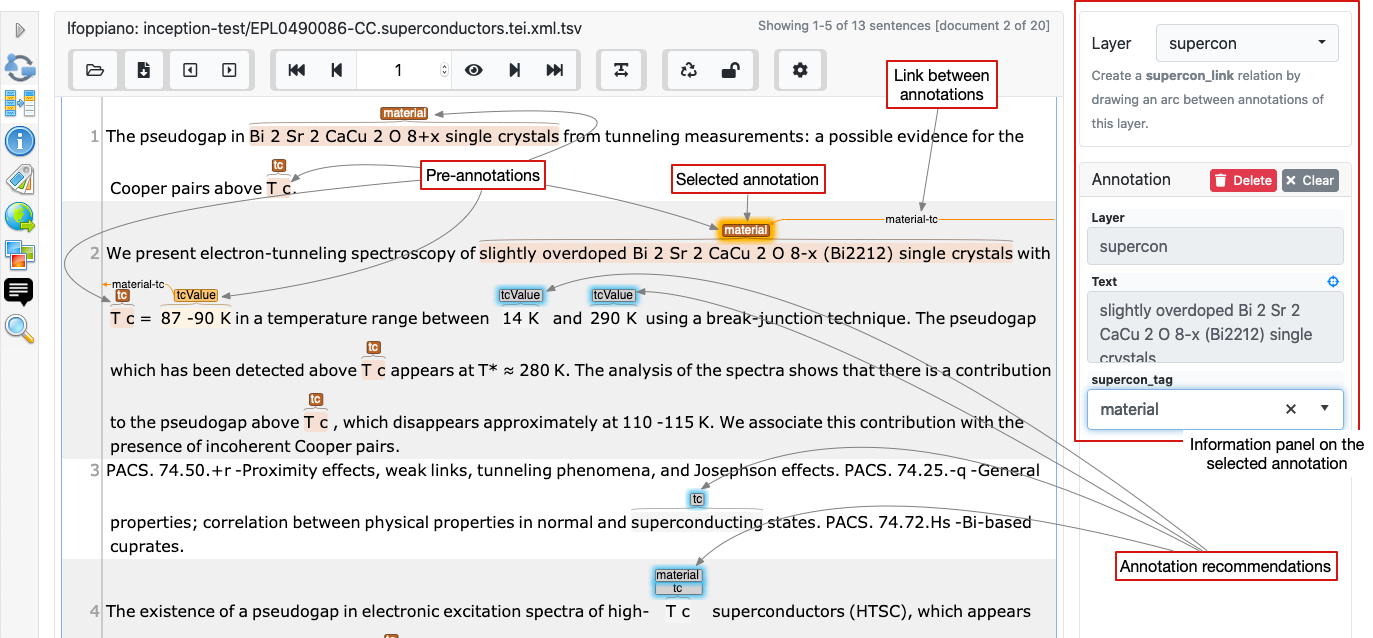
\includegraphics[width=\linewidth]{inception-annotation-interface.png}
%     \captionof{figure}{INCEpTION annotation interface. Annotations and links are visualised in the interface. The interface provides pre-annotations (colored), that were added prior to load the data in the interface and automatic recommendations (grey) which are based on the documents that had been corrected but not yet exported. By clicking on a recommended annotations, the user will validate it and it will be applied to the document. }
%     \label{fig:inception-annotation-interface}
% \end{figure}



% [TODO: revise this part, and reduce it]
% The system was developed as a module of an Open Source machine learning library for TDM processes of scholarly publication: GROBID (Generation of Bibliographic Data)~\cite{GROBID}. 
% GROBID is able to extract, parse and re-structure raw documents such as PDF into structured XML/TEI (Text Encode Initiative)\footnote{https://tei-c.org/} encoded documents with a particular focus on technical and scientific publications. 
% While GROBID provides "low level" scientific documents structures, it allows to develop "high level" modules solving specific tasks on top of it. 
% GROBID provides basics, yet complex functionalities such as a defined structure for text processing, training and evaluation interfaces, the ability to access granular information from the PDF (such as font and styles information, coordinates within the document), and a REST API which simplify the integration with other services. 
% The Grobid ecosystem counts already several modules: grobid-quantities\cite{foppiano2019quantities} for extracting physical quantities, grobid-astro~\footnote{\url{https://github.com/kermitt2/grobid-astro}} for astronomical object recognition, grobid-dictionaries~\cite{grobid-dictionaries} for structuring dictionaries, to mention few of them. 
% The prototype, grobid-superconductors, was implemented combining two different models trained using Conditional Random Field (CRF) ML approach for sequence labelling. 
% Materials names were extracted using a newly built \textit{superconductors} model, and properties values were extracted using grobid-quantities, the Grobid module for physical quantities. The linking between them was performed with a ruled-based approach. 

% We used the prototype evaluation results to define our end to end baseline (described in \cite{foppiano2019proposal}). 
% Results were promising, the system performed well on the entities extraction, although more training data was still necessary. This indicated that a more complete dataset could help not only this project, to develop TDM processes on a larger scope within materials science. 
% We utilised the system was modified to accommodate new labels and it was used for pre-annotation, training and evaluation (\textit{Automatic process} in Figure~\ref{fig:schema-comparison}).




%The designed annotation workflow is composed four main components: the annotation support tools (Section~\ref{subsec:annotation-tool}), the data transformation (Section~\ref{subsec:transformation-of-data}), and the annotation guidelines (Section~\ref{subsec:annotation-guidelines}).

%It’s is very important that all mistakes and information are kept up-to-date in the documentation. In such case, the procedure is to open a new issue in the GitLab issues project page and follow the discussion there. Written discussions will facilitate, in future, the understanding of certain decisions.


% \begin{table}[h]
%     \centering
%     \begin{tabular}{ | c | c | c | } 
%     \hline
%         Block & Sub-block & retained  \\ [0.5ex] 
%     \hline\hline
%         \multirow{5}{4em}{Header} & title & yes\\ 
%             & abstract & yes\\
%             & volume, issn, isbn, doi, journal, .. & no\\
%             & keywords & yes\\
%             & publication, submission dates & no\\
%     \hline
%         \multirow{5}{4em}{Body} & paragraphs & yes\\ 
%             & sections & yes\\
%             & figure caption & yes\\
%             & figure content & no\\
%             & table caption & yes\\
%             & table content & yes\\
%             & equation content & no\\
%             & reference callout & no\\
%     \hline
%         \multirow{2}{4em}{Annex} & paragraphs & yes\\ 
%             & sections & yes\\
%     \hline
%         Bibliographic references & & no\\
%     \hline
%     \end{tabular}
%     \caption{Summary of the information that are retained from a PDF document in the transformation process to the training data XML reference format. "Block" refers to the main document blocks (header, body, annex and bibliographic references). Each of these, is further structured into the Sub-blocks. }
%     \label{table:summary-pdf-data-transformation}
% \end{table}

% \begin{figure}[h]
%     \centering
%     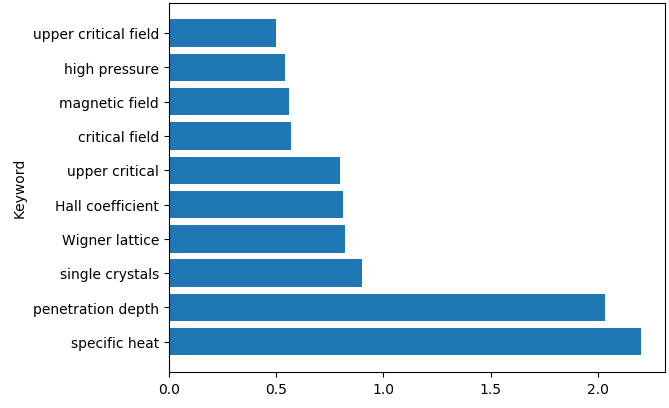
\includegraphics[width=\linewidth]{keyword-top10-body-distribution}
%     \captionof{figure}{Distribution by keyword extracted from the articles body. }
%     \label{fig:keyword-top10-body}
% \end{figure}




% \begin{figure}[h]
%     \centering
%     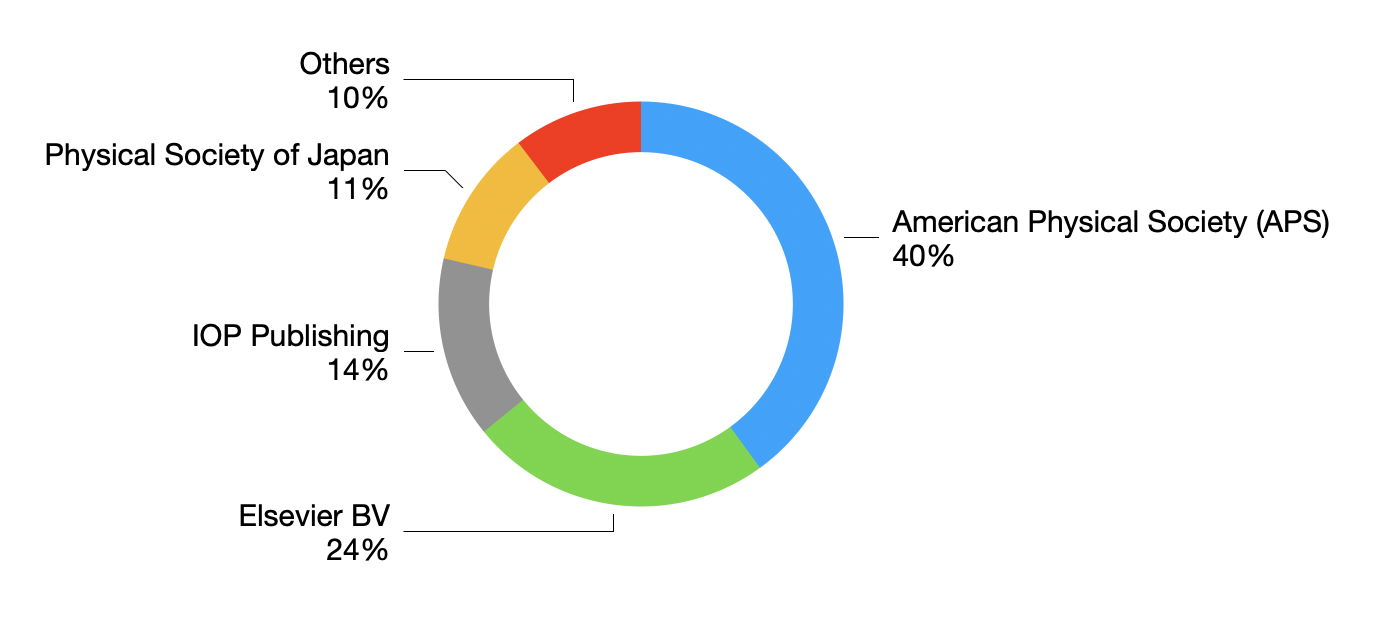
\includegraphics[width=\linewidth]{papes-by-publishers.png}
%     \captionof{figure}{Distribution by publisher automatically extracted from the PDF, and consolidated through lookup to Crossref. }
%     \label{fig:distribution-by-publisher}
% \end{figure}

% \begin{figure}[h]
%     \centering
%     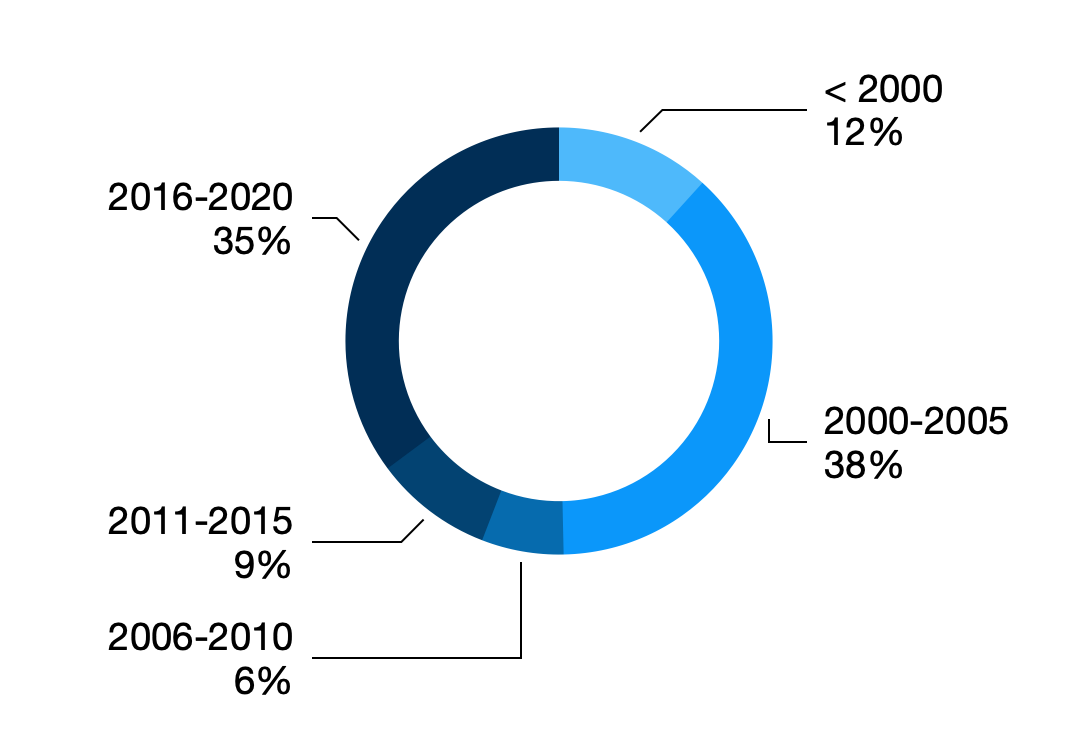
\includegraphics[width=\linewidth]{papers-by-years-donut.png}
%     \captionof{figure}{Distribution by publication year, automatically extracted from the PDF, and consolidated through lookup to Crossref. }
%     \label{fig:distribution-by-year}
% \end{figure}


%[Summarise the approach]
%Initially, a preliminary annotation study on a small number of papers was conducted for domain exploration, to draft and test the annotation process on a smaller scale, and to bootstrap the annotation guidelines.
%Together with domain experts, we then finalised the tag-set and the annotation workflow. 

%The input data, papers related to research in superconductivity, were collected from different sources and publishers.  
%We followed the iterative annotation process of five steps: a) data preparation, b) annotation of relevant entities, c) validation by domain experts, d) test and evaluation, and e) review. 
%The annotation guidelines were, eventually, updated at every iteration. 
%We measured the Inter Annotation Agreement (IAA) using the Krippendorff alpha coefficient~\cite{Krippendorff2004ReliabilityIC} between the annotated (b) and the validated data (c). 
%The obtained results were divided by the level of domain knowledge (domain-experts and non-domain experts) and annotation expertise (novices vs experienced). 
%The aveage IAA, above 0.8, was satisfying. 
%We measured the reliability of the guidelines by reporting that novices annotators with general materials science knowledge could reach a satisfying Inter Annotator Agreement (IAA) in autonomy.

%As a result, we achieved a dataset composed of 145 articles, with 9966 entities (of which, about 4000 unique entities) [TODO: update figures]. They were annotated using six classes: material, class, critical temperature expressions, critical temperature value, critical pressure value and measurement method.
%We added a layer of links between entities, of three types: 1) \textit{material-tc} linking materials and their respective superconducting critical temperature \textit{T\textsubscript{c}}. 
%2) \textit{tc-pressure} connecting \textit{T\textsubscript{c}} and the applied pressure at which it was obtained, and 3) \textit{tc-me\_method} between the critical temperature with the method used to obtain the value of \textit{T\textsubscript{c}}. 
%The superconducting critical temperature is susceptible to conditions such as magnetic field or pressure. 


%In future, we plan to utilise this dataset as training and evaluation data for an automatic database creation system focusing on superconducting materials and their respective properties. 


%The paper is structured as follows: after the introduction, we discuss the methodology used to obtain the data and to produce the final result. Then we describe the information and the validation of the data contained in the dataset. Finally, we provide examples of applications, usability and availability information. 


%SuperMat can be used to support TDM processes for many complementary tasks. 
%such as information retrieval, entity extraction, entity linking, and information clustering.

% The dataset can bee utilised this dataset to train a sequence labelling system, which was then applied to semantically enhance a search engine for scientific documents and a document classification system using superconductors-related classes. 
%The establishment of Text and Data Mining (TDM) processes is an unavoidable step to bridge information collected from scientific literature toward data-driven discovery. 


%The goals of this study were multi-fold: a) definition of a preliminary tag-set schema, b) knowledge acquisition/improvement, c) measuring and monitoring the agreement over several iterative sessions, and d) discovering caveat and problems as soon as possible. 



% \textbf{Entities extraction}: As preliminary evaluation we utilise our corpus for training and evaluating a sequence labelling model for entities recognition using only layouts generated from text (no layout or material information). 
% These results (Table were computed by using 10-fold cross-validation applied to a standard CRF implementation (Wapiti\footnote{\url{https://wapiti.limsi.fr/}}) and a deep learning approach using a Bidirectional LSTM + CRF~\cite{Lample2016NeuralAF} (implemented through DeLFT\footnote{\url{https://github.com/kermitt2/delft}}). 


%Although this dataset has been designed around the superconductors domain, there are considerable overlaps against other domains, for example extracting materials from PDFs for TDM of magnetocaloric materials. 

%\textbf{Material parser}: The data in SuperMat can be used to construct a material parser for unstructured data. 
%The resulting of this application is the ability to recognise various information from a material string, such as structure, formula, name and so on. 
%We will publish the details of this application elsewhere. 


%Lastly, finding documents describing materials belonging to a specific class might be tricky, because the mention of only the class in the document is not a guaranteed that such materials are actually discussed. The solution to this would be to retrieve documents where the class related to the materials entities correspond to the requested class. 
%For example, a search of \textit{cuprate} will find all documents discussing materials that are classified as cuprates by their formula.